\documentclass[tikz,border=8pt]{standalone}
% Shared look for every TikZ diagram. Load with \input{../../tools/tikz-style.tex}
\usepackage[sfdefault]{roboto}
\usetikzlibrary{arrows.meta, positioning, shapes.geometric, calc, fit, backgrounds}
\definecolor{cblue}{HTML}{4C78A8}
\definecolor{corange}{HTML}{F58518}
\definecolor{cgreen}{HTML}{54A24B}
\definecolor{cred}{HTML}{E45756}
\definecolor{cpurple}{HTML}{B279A2}
\definecolor{cgrey}{HTML}{6B6B6B}
\tikzset{
  every picture/.style={font=\sffamily, line width=1.2pt},
  box/.style={draw=#1, fill=#1!12, rounded corners=4pt, align=center, inner sep=7pt, minimum height=1.1cm},
  box/.default=cgrey,
  arrow/.style={-{Stealth[length=3mm]}, draw=cgrey, line width=1.4pt},
  title/.style={font=\sffamily\bfseries\Large},
  note/.style={font=\sffamily\small, text=cgrey, align=center},
}
\AtBeginDocument{\hyphenpenalty=10000 \exhyphenpenalty=10000}

% ROS 1 move_base (one node with a fixed state machine: PLANNING, CONTROLLING, CLEARING; move_base.h, noetic-devel)
% against Nav2 (separate lifecycle servers, ordered by a behaviour tree in bt_navigator; navigation_launch.py, main).
\begin{document}
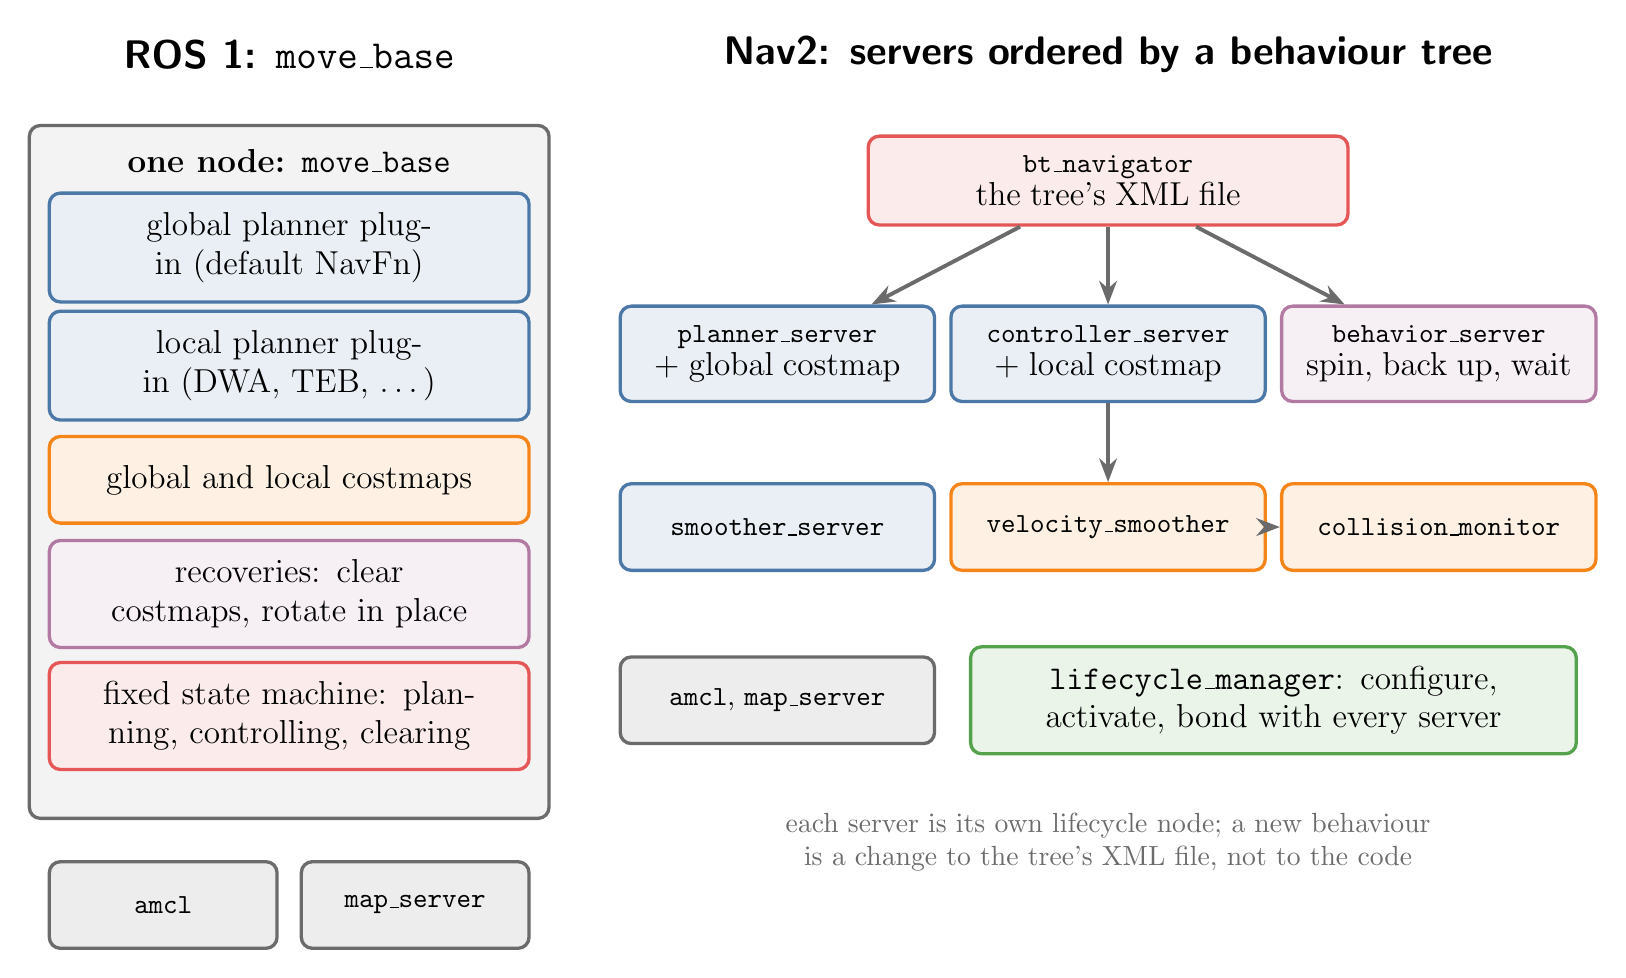
\begin{tikzpicture}[every node/.append style={font=\large}]
  % ---- ROS 1
  \node[title] at (3.2, 10.6) {ROS 1: \texttt{move\_base}};
  \node[draw=cgrey, fill=cgrey!8, rounded corners=4pt, minimum width=6.6cm, minimum height=8.8cm] at (3.2, 5.3) {};
  \node[font=\large\bfseries] at (3.2, 9.25) {one node: \texttt{move\_base}};
  \node[box=cblue, text width=5.6cm] at (3.2, 8.15) {global planner plug-in (default NavFn)};
  \node[box=cblue, text width=5.6cm] at (3.2, 6.65) {local planner plug-in (DWA, TEB, \dots)};
  \node[box=corange, text width=5.6cm] at (3.2, 5.2) {global and local costmaps};
  \node[box=cpurple, text width=5.6cm] at (3.2, 3.75) {recoveries: clear costmaps, rotate in place};
  \node[box=cred, text width=5.6cm] at (3.2, 2.2) {fixed state machine: planning, controlling, clearing};
  \node[box=cgrey, text width=2.4cm, font=\normalsize] at (1.6, -0.2) {\texttt{amcl}};
  \node[box=cgrey, text width=2.4cm, font=\normalsize] at (4.8, -0.2) {\texttt{map\_server}};
  % ---- Nav2
  \node[title] at (13.6, 10.6) {Nav2: servers ordered by a behaviour tree};
  \node[box=cred, text width=5.6cm, font=\normalsize] (bt) at (13.6, 9.0) {\texttt{bt\_navigator}\\ \large the tree's XML file};
  \node[box=cblue, text width=3.5cm, font=\normalsize] (pl) at (9.4, 6.8) {\texttt{planner\_server}\\ \large + global costmap};
  \node[box=cblue, text width=3.5cm, font=\normalsize] (co) at (13.6, 6.8) {\texttt{controller\_server}\\ \large + local costmap};
  \node[box=cpurple, text width=3.5cm, font=\normalsize] (be) at (17.8, 6.8) {\texttt{behavior\_server}\\ \large spin, back up, wait};
  \node[box=cblue, text width=3.5cm, font=\normalsize] (sm) at (9.4, 4.6) {\texttt{smoother\_server}};
  \node[box=corange, text width=3.5cm, font=\normalsize] (vs) at (13.6, 4.6) {\texttt{velocity\_smoother}};
  \node[box=corange, text width=3.5cm, font=\normalsize] (cm) at (17.8, 4.6) {\texttt{collision\_monitor}};
  \node[box=cgrey, text width=3.5cm, font=\normalsize] at (9.4, 2.4) {\texttt{amcl}, \texttt{map\_server}};
  \node[box=cgreen, text width=7.2cm] at (15.7, 2.4) {\texttt{lifecycle\_manager}: configure, activate, bond with every server};
  \draw[arrow] (bt) -- (pl);
  \draw[arrow] (bt) -- (co);
  \draw[arrow] (bt) -- (be);
  \draw[arrow] (co) -- (vs);
  \draw[arrow] (vs) -- (cm);
  \node[note, text width=12cm, font=\normalsize] at (13.6, 0.6) {each server is its own lifecycle node; a new behaviour is a change to the tree's XML file, not to the code};
\end{tikzpicture}
\end{document}
